\documentclass[11pt]{article}

\oddsidemargin=0in
\evensidemargin=0in
\textwidth=6.3in
\topmargin=-0.5in
\textheight=9in

\parindent=0in
%\pagestyle{empty}



%------------------------------------------------------------------
% PROBLEM, PART, AND POINT COUNTING...

% Create the problem number counter.  Initialize to zero.
\newcounter{problemnum}

% Specify that problems should be labeled with arabic numerals.
\renewcommand{\theproblemnum}{\arabic{problemnum}}


% Create the part-within-a-problem counter, "within" the problem counter.
% This counter resets to zero automatically every time the PROBLEMNUM counter
% is incremented.
\newcounter{partnum}[problemnum]

% Specify that parts should be labeled with lowercase letters.
\renewcommand{\thepartnum}{\alph{partnum}}

% Make a counter to keep track of total points assigned to problems...
\newcounter{totalpoints}

% Make counters to keep track of points for parts...
\newcounter{curprobpts}		% Points assigned for the problem as a whole.
\newcounter{totalparts}		% Total points assigned to the various parts.

% Make a counter to keep track of the number of points on each page...
\newcounter{pagepoints}
% This counter is reset each time a page is printed.

% This "program" keeps track of how many points appear on each page, so that
% the total can be printed on the page itself.  Points are added to the total
% for a page when the PART (not the problem) they are assigned to is specified.
% When a problem without parts appears, the PAGEPOINTS are incremented directly
% from the problem as a whole (CURPROBPTS).


%---------------------------------------------------------------------------


% The \problem environment first checks the information about the previous
% problem.  If no parts appeared (or if they were all assigned zero points,
% then it increments TOTALPOINTS directly from CURPROBPTS, the points assigned
% to the last problem as a whole.  If the last problem did contain parts, it
% checks to make sure that their point values total up to the correct sum.
% It then puts the problem number on the page, along with the points assigned
% to it.

\newenvironment{problem}[1]{
% STATEMENTS TO BE EXECUTED WHEN A NEW PROBLEM IS BEGUN:
%
% Increment the problem number counter, and set the current \ref value to that
% number.
\refstepcounter{problemnum}
%
% Add some vspace to separate from the last problem.
\vspace{0.15in} \par
%
\setcounter{curprobpts}{#1} \setcounter{totalparts}{0}	% Reset counters.
%
% Now put in the "announcement" on the page.
{\Large \bf \theproblemnum. \normalsize ({\it \arabic{curprobpts} point\null\ifnum \value{curprobpts} = 1\else s\fi}\/)}
}{
% STATEMENTS TO BE EXECUTED WHEN AN OLD PROBLEM IS ENDED:
%
% If no parts to problem, then increment TOTALPOINTS and PAGEPOINTS for the
% entire problem at once.
\ifnum \value{totalparts} = 0
	\addtocounter{totalpoints}{\value{curprobpts}}	% Add pts to total.
	\addtocounter{pagepoints}{\value{curprobpts}}	% Add pts to page total.
%
% If there were parts for the problem, then check to make sure they total up
% to the same number of points that the problem is worth. Issue a warning
% if not.
\else \ifnum \value{totalparts} = \value{curprobpts}
	\else \typeout{}
	\typeout{!!!!!!!   POINT ACCOUNTING ERROR   !!!!!!!!}
	\typeout{PROBLEM [\theproblemnum] WAS ALLOCATED \arabic{curprobpts} POINTS,}
	\typeout{BUT CONTAINS PARTS TOTALLING \arabic{totalparts} POINTS!}
	\typeout{}
	\fi
\fi
}


%---------------------------------------------------------------------------


% The \newpart command increments the part counter and displays an appropriate
% lowercase letter to mark the part.  It adds points to the point counter
% immediately.  If 0 points are specified, no point announcement is made.
% Otherwise, the announcement is in scriptsize italics.

\newcommand{\newpart}[1]
{
\refstepcounter{partnum}	% Set the current \ref value to the part number.
\hspace{0.25in}		% Indent the part by a quarter inch.
%
% If points are to be printed for this problem (signaled by point value > 0),
% then put them in in scriptsize italics.
\ifnum #1 > 0
	\makebox[0.5in][l]{{\bf \thepartnum.} {\bf ({\it #1 pt\ifnum #1 = 1\else s\fi\/}) \,\,}}
\else
	\makebox[0.25in][l]{({\bf \thepartnum})}
\fi
%
\hspace{0.1in}		% Lead the material away from the part "number".
%
\addtocounter{totalparts}{#1}	% Add points to totalparts for this problem.
\addtocounter{pagepoints}{#1}	% Add points to total for this page.
\addtocounter{totalpoints}{#1}	% Add points to total for entire test.
}


%---------------------------------------------------------------------------



% Just in case you want to skip some numbers in your test...

\newcommand{\skipproblem}[1]{\addtocounter{problemnum}{#1}}



%---------------------------------------------------------------------------


% The \showpoints command simply gives a count of the total points read in up to
% the location at which the command is placed.  Typically, one places one
% \showpoints command at the end of the latex file, just prior to the
% \end{document} command.  It can appear elsewhere, however.

\newcommand{\showpoints}
{
\typeout{}
\typeout{====> A TOTAL OF \arabic{totalpoints} POINTS WERE READ.}
\typeout{}
}


%---------------------------------------------------------------------------



\usepackage{graphicx}
\usepackage[english]{babel}
\usepackage[latin1]{inputenc}
\usepackage{times}
\usepackage[T1]{fontenc}
\usepackage{amsmath}
\usepackage{amssymb}
\usepackage{subfigure}

\newcommand{\argmax}{\mathop{\arg\max}}
\newcommand{\deriv}[1]{\frac{\partial}{\partial {#1}} }
\newcommand{\dsep}{\mbox{dsep}}
\newcommand{\Pa}{\mathop{Pa}}
\newcommand{\ND}{\mbox{ND}}
\newcommand{\De}{\mbox{De}}
\newcommand{\Ch}{\mbox{Ch}}
\newcommand{\graphG}{{\mathcal{G}}}
\newcommand{\graphH}{{\mathcal{H}}}
\newcommand{\setA}{\mathcal{A}}
\newcommand{\setB}{\mathcal{B}}
\newcommand{\setS}{\mathcal{S}}
\newcommand{\setV}{\mathcal{V}}
\DeclareMathOperator*{\union}{\bigcup}
\DeclareMathOperator*{\intersection}{\bigcap}
\DeclareMathOperator*{\Val}{Val}
\newcommand{\mbf}[1]{{\mathbf{#1}}}
\newcommand{\eq}{\!=\!}

\newcommand{\discrete}{stripes}
\newcommand{\gaussian}{swirl}

\begin{document}

{\centering
  \rule{6.3in}{2pt}
  \vspace{1em}
  {\Large
    CS688: Graphical Models - Spring 2014\\
    Assignment 3\\
  }
  \vspace{1em}
  Assigned: Thursday, Mar 13th. Due: Thursday, Mar 27th 2:30pm\\
  \vspace{0.1em}
  \rule{6.3in}{1.5pt}
}\vspace{1em}

\textbf{General Instructions:} Submit a report with the answers to each question at the start of class on the date the assignment is due. You are encouraged to typeset your solutions. To help you get started, the full \LaTeX source of the assignment is included with the assignment materials. For your assignment to be considered ``on time'', you must upload a zip file containing all of your code to Moodle by the due date. Make sure the code is sufficiently well documented that it's easy to tell what it's doing. You may use any programming language you like. For this assignment, you may \textbf{not} use existing code libraries for inference and learning with CRFs or MRFs. If you think you've found a bug with the data or an error in any of the assignment materials, please post a question to the Moodle discussion forum. Make sure to list in your report any outside references you consulted (books, articles, web pages, etc.) and any students you collaborated with.\\

\textbf{Academic Honesty Statement:} Copying solutions from external sources (books, web pages, etc.) or other students is considered cheating. Sharing your solutions with other students is also considered cheating. Any detected cheating will result in a grade of 0 on the assignment for all students involved, and potentially a grade of F in the course.\\

\textbf{Introduction:} In this assignment, you will experiment with Monte Carlo image denoising using grid-structured conditional random field models. We will consider both discrete random fields for binary images and Gaussian random fields for real-valued images.\\

\textbf{Data Set:} The data for this assignment consists of two $100 \times 100$ pixel images. The \textit{\discrete} image is a binary image for use with the discrete model with pixel values that are either $0$ or $1$. The original image is \textit{\discrete.txt}, while the copy with noise added in \textit{\discrete-noise.txt}. The \textit{\gaussian} image is a real-valued image with pixels values in the range $[0,1]$ for use with the Gaussian model. The original image is \textit{\gaussian.txt}, while the copy with noise added in \textit{\gaussian-noise.txt}.
The four images are shown below. We will refer to the images without noise as the ``true" images and the images with noise as the ``observed" or ``noisy" images.

\begin{figure}[ht]
\centering
\subfigure[\discrete]{
   \includegraphics[width=1.4in] {Figures/\discrete.png}
 }
 \subfigure[\discrete-Noise]{
   \includegraphics[width=1.4in] {Figures/\discrete-noise.png}
 }
 \subfigure[\gaussian]{
   \includegraphics[width=1.4in] {Figures/\gaussian.png}
 }
 \subfigure[\gaussian-Noise]{
   \includegraphics[width=1.4in] {Figures/\gaussian-noise.png}
 }
\end{figure}



\textbf{Models: } We will consider a grid-structured CRF model with two sets of variables $\mbf{Y}$ and $\mbf{X}$. $X_{ij}$ will represent the value of pixel $(i,j)$ in the observed, noisy image. $Y_{ij}$ will represent the de-noised value of pixel $(i,j)$.  We will denote the pixels of the true image by $I_{ij}$. We will let $W$ represent the width of the image and $H$ represent the height. The CRF model connects each pixel variable $Y_{ij}$ in the de-noised image to it's nearest neighbors in the de-noised image. Its nearest neighbors are the pixels directly above, below, left and right of location $(i,j)$. Pixels on the border of the image will have two or three neighbors, while  pixels off the border of the image will have four neighbors. Each de-noised pixel variable  $Y_{ij}$ is also connected to the corresponding pixel in the noisy image $X_{ij}$. Each edge in the graph is associated with a pairwise potential. The graph structure is shown below.\\

\begin{figure}[ht]
\centering
   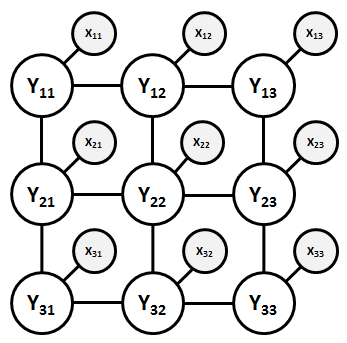
\includegraphics[width=3in] {Figures/grid-crf.png}
\end{figure}

We let $V$ denote the set of pixel locations in the image and $E$ denote the set of neighboring pixel locations. Since a pixel location is a pair $(i,j)$, the set $V$ contains pairs $(i,j)$. $E$ thus contains pairs of pixel locations $(i,j),(k,l)$ that are neighbors in the graph. \\

The conditional distribution over de-noised pixel values given noisy pixel values for the binary case is given below. The set $\mathcal{Y}$ is the joint domain of the de-noised pixel variables $Y_{ij}$. For a binary image of size $W\times H$, this is $\{0,1\}^{W\times H}$.

\begin{align}
P(\mbf{Y}=\mbf{y}|\mbf{x}) &= \frac{\displaystyle \exp\left(\sum_{(i,j),(k,l)\in E} W^P_{ijkl}[y_{ij}=y_{kl}] +  \sum_{(i,j) \in V} W^L[y_{ij}=x_{ij}] \right)}
{\displaystyle\sum_{\mbf{y}\in\mathcal{Y}}\exp\left(\sum_{(i,j),(k,l)\in E} W^P_{ijkl}[y'_{ij}=y'_{kl}] +  \sum_{(i,j) \in V} W^L[y'_{ij}=x_{ij}]^2\right) }
\end{align}

The conditional distribution over de-noised pixel values given the noisy pixel values for the Gaussian case is given next. The set $\mathcal{Y}$ is the joint domain of the de-noised pixel variables $Y_{ij}$. For an image of size $W\times H$ with real-valued pixels, this is $\mathbb{R}^{W\times H}$.

\begin{align}
P(\mbf{Y}=\mbf{y}|\mbf{x}) &= \frac{\displaystyle \exp\left(-\sum_{(i,j),(k,l)\in E} W^P_{ijkl}(y_{ij}-y_{kl})^2 -  \sum_{(i,j) \in V} W^L(y_{ij}-x_{ij})^2 \right)}
{\displaystyle\int_{\mathcal{Y}}\exp\left(-\sum_{(i,j),(k,l)\in E} W^P_{ijkl}(y'_{ij}-y'_{kl})^2 -  \sum_{(i,j) \in V} W^L(y'_{ij}-x_{ij})^2\right)d\mbf{y}' }
\end{align}

Both models trade off smoothness in the de-noised image (the first terms) against the degree to which the de-noised image looks like the noisy image (the second terms). When the pairwise weights $W^P_{ijkl}$ are large, the model favors smoothness, when the local weight $W^L$ is large, the model favors being close to the noisy image. In the most general case, we can consider a different amount of smoothing between every pair of de-noised variables $Y_{ij}$ and $Y_{kl}$ as given by $W^P_{ijkl}$. To begin, we will consider the special case where all the $W^P_{ijkl}$'s are equal to the same value $W^P$.\\

\textbf{Algorithm:} To de-noise the observed image $\mbf{X}$, we perform inference in the CRF model to compute the posterior mean of each de-noised pixel variable $Y_{ij}$ conditioned on the noisy pixel values $\mbf{x}$. The graph is strongly loopy, so we will use a particle-based approximation. Specifically, we will use $T$ iterations of the Gibbs sampler. The Gibbs sampler operates by cycling over each variable $Y_{ij}$ and sampling a new value for that variable from its conditional distribution given the current values of the other variables in its Markov blanket. The Markov blanket of a variable $Y_{ij}$ consists of it's neighbors $Y_{kl}$ in the grid, and the noisy pixel variable $X_{ij}$.\\

For the binary model, the conditional distribution is easy to obtain from first principles. We use $\mbf{A}_{ij}$ to denote the set of neighbors of $Y_{ij}$ in the grid and $\mbf{y}_{\mbf{A}_{ij}}$ to denote the values of the neighbors.

\begin{align}
P(Y_{ij}=1|\mbf{y}_{\mbf{A}_{ij}},x_{ij}) &= \frac{\displaystyle \exp\left(
\sum_{(k,l)\in A_{ij}} W^P[y_{kl}=1] + W^L[x_{ij}=1] \right)}
{\displaystyle \sum_{y=0}^1\exp\left(
\sum_{(k,l)\in A_{ij}} W^P[y_{kl}=y] + W^L[x_{ij}=y] \right)}
\end{align}

The Gibbs sampler starts by assigning an initial value to each $Y_{ij}$. We can simply set $y_{ij}=x_{ij}$. On each iteration $t$, the Gibbs sampler sweeps through all variables $Y_{ij}$, updating their values one at a time. The Gibbs sampler updates the value of $Y_{ij}$ by drawing a random sample from the conditional distribution $P(Y_{ij}=1|\mbf{y}_{\mbf{A}_{ij}},x_{ij})$, which is a simple Bernoulli distribution. We can do this by drawing a uniform random number $\alpha$ on $[0,1]$ and setting  $y_{ij}=1$ if $\alpha < P(Y_{ij}=1|\mbf{y}_{\mbf{A}_{ij}},x_{ij})$ and setting $y_{ij}=0$ otherwise. After sweeping through all pixel locations on iteration $t$,  we set $y^t_{ij}=y_{ij}$ to save the sample. The estimate for the de-noised pixel values after $t$ iterations is the particle approximation to the posterior mean given by $\bar{y}_{ij} = \frac{1}{t}\sum_{s=1}^ty^s_{ij}$.
\\

In the Gaussian case, the conditional distribution of $Y_{ij}$ given $\mbf{y}_{\mbf{A}_{ij}}$ and $x_{ij}$ can also be obtained in closed form, although the derivation is somewhat more difficult.

\begin{align}
P(Y_{ij}=y|\mbf{y}_{\mbf{A}_{ij}},x_{ij}) &\propto  \exp\left(-\sum_{(k,l)\in A_{ij}} W^P(y_{kl}-y)^2 - W^L(x_{ij}-y)^2 \right)
\end{align}

We can see that up to normalization, the conditional distribution is the exp of the negative of a sum of several quadratic terms in involving $y$. This is exactly the form of an unnormalized univariate normal distribution, so we need only work out the mean and standard deviation of the distribution. We let $N_{ij}$ denote the number of neighbors of $Y_{ij}$ in the grid, expand the quadratic forms to identify the coefficients of $y^2$ and $y$, and drop additional terms that don't depend on $y$.

\begin{align}
P(Y_{ij}=y|\mbf{y}_{\mbf{A}_{ij}},x_{ij}) &\propto  \exp\left(- y^2(W^PN_{ij} + W^L) +  2y\left(W^Lx_{ij} + \sum_{(k,l)\in A_{ij}} W^Py_{kl}\right) \right)
\end{align}

In a normal distribution with mean $\mu_{ij}$ and standard deviation $\sigma_{ij}$, we have that:

\begin{align}
\mathcal{N}(y|\mu_{ij},\sigma_{ij}) &\propto  \exp\left(-\frac{1}{2\sigma_{ij}^2}(y-\mu_{ij})^2\right)
\propto  \exp\left(-y^2\frac{1}{2\sigma_{ij}^2} +y\frac{1}{\sigma_{ij}^2}\mu_{ij}\right)
\end{align}

By matching the coefficients in the two distributions, we can see that:

\begin{align}
-y^2\frac{1}{2\sigma_{ij}^2} &= - y^2(W^PN_{ij} + W^L)\\
\sigma^2_{ij} &= \frac{1}{2(W^PN_{ij} + W^L)}\\
&\\
y\frac{1}{\sigma_{ij}^2}\mu_{ij} &= 2y\left(W^L x_{ij} + \sum_{(k,l)\in A_{ij}} W^Py_{kl}\right)\\
\mu_{ij}&=2\sigma_{ij}^2\left(W^Lx_{ij} + \sum_{(k,l)\in A_{ij}} W^Py_{kl}\right)\\
&=\frac{1}{W^PN_{ij} + W^L}\left(W^Lx_{ij} + \sum_{(k,l)\in A_{ij}} W^Py_{kl}\right)
\end{align}

We apply the Gibbs sampler to the Gaussian CRF model in exactly the same way that we apply it to the discrete CRF model. We initialize all of the $Y$ variables to $y_{ij}=x_{ij}$. On each iteration $t$ we sweep through all pixel locations $(i,j)$ in the image. For each pixel location, we sample $y_{ij}$ from its conditional distribution given the current values of the neighboring variables in the grid $y_{kl}$, $(k,l)\in A_{ij}$ and the noisy observed pixel $x_{ij}$. As shown above, this conditional distribution on $y_{ij}$ is a univariate normal distribution. We use the formulas above to compute the mean $\mu_{ij}$ and variance $\sigma^2_{ij}$ of this conditional distribution. To sample a value for $y_{ij}$, we first use a library function to draw a random standard normal value $z\sim \mathcal{N}(z|0,1)$. We then set $y_{ij} = \mu_{ij} + z\sqrt{\sigma^2_{ij}}$, which is a draw from $\mathcal{N}(y_{ij}|\mu_{ij},\sigma^2_{ij})$. After sweeping through all pixel locations on iteration $t$,  we set $y^t_{ij}=y_{
ij}$ to save the sample. Our estimate for the de-noised pixel values after $t$ iterations is again the particle approximation to the posterior mean given by $\bar{y}_{ij} = \frac{1}{t}\sum_{s=1}^ty^s_{ij}$.



\begin{problem}{40} \textbf{Monte Carlo De-noising for Binary Images:}
Implement the Gibbs sampling procedure for the binary CRF model as described above and use your implementation to perform the following exercises:
\\

\textbf{(a)} Select positive values for $W^P$ and $W^L$ and run your Gibbs sampler for $T=100$ iterations on the \textit{\discrete-noise} image. Compute the posterior mean image $\bar{y}$ using the $T$ samples from your Gibbs sampler as described above. Compute the mean absolute error between the pixels in the posterior mean image $\bar{y}$ and the pixels in the true \textit{\discrete} image $I$. The MAE is defined to be $(1/HW)\sum_{(i,j)}|\bar{y}_{ij} - I_{ij}|$. Try different values of $W^P$ and $W^L$ and determine values that give good performance in terms of MAE. Report the values of the parameters $W^P$ and $W^L$ that you find and the corresponding MAE. Display the best posterior mean image $\bar{y}$ that you find, along with posterior mean images for settings of $W^P$ and $W^L$ that resulted in over and under-smoothing.\\

\textbf{(b)} Using the best parameters you found in part \textbf{(a)}, again run the Gibbs sampler until the MAE converges. On each iteration, compute the $t$-step posterior mean image $\bar{y}$ using samples $1$ to $t$. Compute the MAE between the $t$-step posterior mean image and the true image $I$. Produce a plot showing the MAE of the $t$-step posterior mean images versus $t$. How many iterations does it take for the posterior mean MAE to converge?
\end{problem}


\begin{problem}{60} \textbf{Monte Carlo De-noising for Real-Valued Images:}
Implement the Gibbs sampling procedure for the Gaussian CRF model as described above and use your implementation to perform the following exercises:
\\

\textbf{(a)} Apply your Gibbs sampler to the \textit{\gaussian-noise} image and identify values for $W^P$ and $W^L$ that give good de-noising performance in terms of MAE. Report the parameters and the corresponding MAE value. Display the posterior mean image $\bar{y}$ found using these parameters.\\

\textbf{(b)} As we will see shortly, the general case of a different pairwise weight $W^P_{ijkl}$ for every pair of neighboring pixel locations $(i,j)$ and $(k,l)$ is very useful. Re-derive the mean and variance of the conditional distribution on $y_{ij}$ using the more general form of the weights $W^P_{ijkl}$. Report the modified mean and variance formulas. Show some work.\\

\textbf{(c)} One of the main problems with the basic Gaussian model is that it smooths strong image edges along with noise. Intuitively, when the squared difference between the noisy pixel values $(x_{ij}-x_{kl})^2$ is large, we don't want the model to assert that $(y_{ij}-y_{kl})^2$ should be small. We can achieve this effect by setting the general pairwise weights $W^P_{ijkl}$ to $\frac{W^P}{0.01+(x_{ij}-x_{kl})^2}$, where $W^P$ is a global pairwise weight parameter. Implement the Gibbs sampler using general pairwise weights $W^P_{ijkl}$ using the mean and variance you found in \textbf{(b)}
Explore values of $W^P$ and $W^L$, computing the general pairwise weights $W^P_{ijkl}$ using the above formula with each value of $W^P$. Identify values of $W^P$ and $W^L$ that perform well on \textit{\gaussian-noise} in terms of MAE. Report the MAE, the values of the weights and display the de-noised image. Do you obtain better MAE with the basic or more general model? Which model leads to de-noised images that are visually less noisy?

\end{problem}

\showpoints
\end{document} 